\documentclass{article} % For LaTeX2e
\usepackage{cos424,times}
\usepackage{hyperref}
\usepackage{url}
\usepackage{graphicx}
\usepackage{amsmath}
%\usepackage{natbib}
\usepackage{multirow}
\usepackage{bm,bbm}
 \usepackage{amssymb}
 \title{Fast classification of newsgroup posts}


\author{
Barbara E Engelhardt\\
Department of Computer Science\\
Princeton University\\
\texttt{bee@princeton.edu} \\
%\And
%Coauthor \\
%Affiliation \\
%\texttt{email} \\
}

\newcommand{\fix}{\marginpar{FIX}}
\newcommand{\new}{\marginpar{NEW}}

\begin{document}

\maketitle

\begin{abstract}
Streaming text data is ubiquitous: Google News, Twitter, Facebook, and many other websites have large numbers of posts from users every second. Often, we would like to classify these posts into specific categories as they arrive in order to organize the many new posts for other users to filter efficiently. In this assignment, we address the problem of classifying newsgroup posts using a number of different feature sets and methods for classification. We evaluate these methods on the 20 Newgroups data set, which contains 20,000 posts to twenty different newsgroups, where the newsgroup labels each post into each of twenty distinct classes. We train the classifiers on bag-of-words representations of each post, with and without feature selection. We find that decision trees and random forest classifiers uniformly have the highest precision and recall, whereas the perceptron and hinge loss perform poorly with respect to the other classifiers.
\end{abstract}
\section{Introduction}

The need for classifying streaming text is everywhere. The Associated Press releases articles that need to be filed under specific headings in Google News. Twitter and Facebook analyze each post in real time. Emails arrive in our inbox and must be filtered into \emph{Spam} or \emph{Inbox}. We are interested in understanding which classification methods perform well on this task. Furthermore, we would like to understand the properties of a classifier that are useful in performing this task in order to consider developing new classifiers for this purpose.

In this work, we evaluate ten separate classification methods in the task of classifying newsgroup categories from posts. For this task, we have modeled the posts using a bag-of-words representation. We evaluated the performance of each of the classification methods with and without feature selection to quantify the benefits of feature selection on classifier performance and also on the computational speed of each of the classifiers.

\section{Related Work}

This data set is the canonical text multi class classification data set in the machine learning community, and has been used as a benchmark for text classification methods in many contexts. In particular, recent text classification methods have used the bag-of-words representation of this data set projected down to a set of latent \emph{topics}, where the projection is informed by the class label~\cite{zhu2009,lacoste2009}. Then, for testing, new posts also are considered in the context of the low-dimensional topic space instead of their bag-of-words representation. This suggests that feature selection may benefit the classification task.


\subsection{Data processing}

We downloaded the 20 Newsgroups data set on January 5th, 2015 from the UCI Machine Learning Archive~\footnote{{\tt http://kdd.ics.uci.edu/}}. We used the Python NLTK library to tokenize, convert to lower case, remove stop words, lemmatize, stem each word using the Porter stemming method, and filtering words that occurred fewer than $200$ times in the corpus~\cite{bird2009}. The resulting vocabulary contained $3,256$ words. We converted these words to the bag-of-words format as features of the posts; we used the newsgroup name that each document was posted to as its label. We considered the effect of feature selection on the classifiers, where feature selection is performed using a support vector machine with a linear kernel and $\ell_1$ penalty. After feature selection, we were left with $488$ dictionary words in the bag-of-words representation, which is $15\%$ of the original feature set size.

\subsection{Classification methods}

We use ten different classification methods from the SciKitLearn Python libraries~\cite{scikit-learn}. All parameterizations are the default unless specified.
\begin{enumerate}
\item \emph{$K$-nearest neighbors} (KNN): using ten nearest neighbors and the ``KDTree" algorithm
\item \emph{Logistic regression with $\ell_2$ penalty} (LR): using stochastic gradient descent 
\item \emph{Perceptron with $\ell_2$ penalty} (P2): using stochastic gradient descent
\item \emph{Hinge loss with $\ell_2$ penalty} (HL2): using stochastic gradient descent
\item \emph{Naive Bayes classifier} (NB): using multinomial implementation
\item \emph{Support vector machine with linear kernel} (SVML): 
\item \emph{Support vector machine with squared exponential kernel} (SVMS): 
\item \emph{AdaBoost} (AB): using $100$ estimators
\item \emph{Decision tree} (DT): using Gini impurity scores 
\item \emph{Random forest} (RF): using Gini impurity scores and 100 trees
\end{enumerate}

Because this problem is one of multiclass classification, we trained and tested each of these classifiers as binary classifiers for each class using one-versus-rest classification; for this we also used the SciKit-Learn library. Because there were equal numbers of samples in each class, we averaged the evaluation metrics across the twenty classes for the values across the $20$ newsgroups.

\subsection{Evaluation}

For each classification method, we performed stratified 10-fold cross validation on the 20 Newsgroups data. We maintained the same folds across each of the classifiers. We compared the different classifier results using precision, false discovery rate (FDR), $F_1$ score, and wall clock time in seconds, all of which were averaged over the results from each of the 20 classes (each of which had identical numbers of posts). In particular, denoting the number of false positives (FPs), true positives (TPs), false negatives (FNs), true negatives (TNs), and false discovery rate (FDR), we can define precision and recall as
\begin{equation*}
\mbox{precision} = \frac {TP}{TP+FP} = 1 - FDR \mbox{,  recall} = \frac {TP}{TP+FN}
\end{equation*}
and $F_1$-score, which is the harmonic mean of precision and recall:
\begin{equation*}
F_1 = 2 \frac {precision \times recall} {precision + recall} = 2 \frac{TP}{2TP+FP+FN}.
\end{equation*}
\newpage
\section{Spotlight Classifier: Perceptron Algorithm}

%\subsection{Overview}

The perceptron (Rosenblatt, 1958), is a linear classfication algorithm that forms the foundation of many modern discriminative models. Given a dataset $\mathcal{D} = \{(\bm{x}_1,t_1),(\bm{x}_2,t_2)...(\bm{x}_N,t_N)\}$, where  $\bm{x}\in \mathbb{R}^d$ are the $d$-dim input feature vectors and $t \in \{-1,+1\}$ are the true labels, the perceptron algorithm learns the following generalized linear model:

$\quad \qquad \qquad \qquad \qquad \qquad \qquad \qquad \qquad y(\bm{x}) = f(\bm{w}^T\bm{x})$

Here, $y(\bm{x})$ are the predicted labels, the model is parameterized by the weight vector $\bm{w} \in \mathbb{R}$, and $f$ is some nonlinear activation function, such as softmax, tanh or the step function, given by:

$ \qquad \qquad \qquad \qquad \qquad \qquad \qquad f(x) = \begin{cases} +1 & x \geq 0 \\ -1 & x<0 \\ \end{cases}$

The algorithm used to learn the parameters $\bm{w}$ of the perceptron can most easily be motivated by error function minimization. The simplest formulation of this would be minimixing the number of misclassified samples, but this does not yield a simple gradient based learning algorithm because the error is a piecewise constant function of $\bm{w}$, with discontinuities wherever a change in $\bm{w}$ causes the decision boundary to move across one of the data points. \cite{bishop2006pattern}

$\qquad \qquad \qquad ${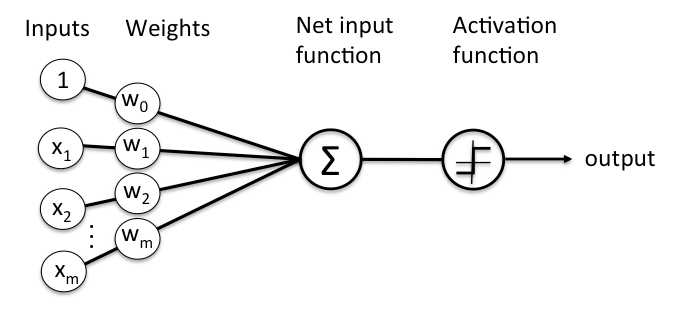
\includegraphics[width=0.7\textwidth]{perceptron.png}}

We use instead the perceptron criterion (a modified version of hinge loss, with the `hinge' at $x=0$):

{$\qquad \qquad \qquad \qquad \qquad \qquad \qquad E_P(\bm{w}) = -\sum\limits_{n=1}^N \min(0, \bm{w}^T\bm{x}_nt_n) $}

If the predicted label matches the true label for sample $n$, $(\bm{w}^T\bm{x}_n)\cdot t_n > 0$. The perceptron criterion therefore
associates zero loss for correct classification, while for a misclassified sample, it tries to minimize $\bm{w}^T\bm{x}_nt_n)$.

%\subsection{Training}
The algorithm for learning the weights of a perceptron is as follows:
\begin{enumerate}

\item[(1)] Initialize weights of the perceptron $w^{(0)}$

\item[(2)] At iteration $i$, for each sample $n = 1...N$: 

- Evaluate predictions $y(\bm{x}_n) = f(\bm{w}^{(i)T}\bm{x}_n)$

- Update weights according to the :
$ \bm{w}^{(i+1)} = \bm{w}^{(i)} + (t_n - y(\bm{x}_n))\bm{x}_n $

\item[(3)] Repeat (2) until convergence (e.g. until iteration error is below some defined threshold)

\end{enumerate}

%\subsection{Evaluating classifier}

The perceptron algorithm is guaranteed to converge, provided the data is linearly separable, i.e., that there exist parameters $\bm{w}$ that achieves 0 error on the training set. If the data is not linearly separable however, the algorithm will not converge, or will take a very long time. 

The algorithm can easily be framed in an online setting, iteratively updating weights with each new sample. Also, unlike other logistic regression, etc, there is no need to set a learning rate (multiplying the update by a constant would simply rescale the weights, and has no effect on the predicted label).

%The algorithm can be used to fit models where computing marginals $p(y|x,w)$ is more expensive than computing the MAP output, $\text{argmax}_y\, p(y|x,w)$; this arises in some structured-output classification problems.

\newpage

\section{Results}

\subsection{Evaluation results}

We found variable performance of each of the ten classifiers on the 20 Newsgroups data, particularly with respect to recall (Table~\ref{tab:classifiers}). In particular, we see that the linear classifiers (LR, P2, HL2, NB, and SVML) tend to perform worse on this task on average relative to the non-linear classifiers (AB, SVMS, DT, RF), although logistic regression has strong performance for a linear classifier. Of the non-linear classifiers, the AdaBoost, random forest, and decision tree classifiers have stronger performance than the SVMS. Overall, the decision tree shows competitive performance, despite its simplicity relative to the other nonlinear methods. This suggests that it is a non-additive combination of the word counts, rather than either a very high dimensional basis function (SVMS) or ensemble classifiers (RF, AdaBoost), that creates the biggest gains in performance over linear classifiers.

\begin{table}[htbp]
\small
   \centering
   \begin{tabular}{@{}|c|c|c|c|c|c|c|c|c|@{}} % Column formatting, @{} suppresses leading/trailing space 
   \hline
    &  \multicolumn{4}{c}{No feature selection} &
  \multicolumn{4}{c|}{Feature selection}  \\
  \cline{2-9}
   Classifier & Prec & Recall & $F_1$ & Time (s)& Prec & Recall & $F_1$ & Time (s) \\ \hline \hline
      KNN   &  0.77 & 0.34 & 0.45 & 1480.4 & 0.74 & 0.40 & 0.54 & 272.1\\
        LR   &  0.81 & 0.89 & 0.85 & 23.7& 0.76 & 0.91 & 0.82 & 14.8 \\
      P2      &  0.68 & 0.22 & 0.25 & 5.99& 0.66 & 0.20 & 0.21 & 0.98\\
      HL2    &  0.70 & 0.22 & 0.24 & 6.04& 0.66 & 0.19 & 0.19 & 0.97 \\
      NB &  0.39 & 0.94 & 0.53 & 4.34& 0.36 & 0.95 & 0.50 & 0.69  \\
      SVML &  0.78 & 0.90 & 0.83 & 11.1 & 0.65 & 0.90 & 0.75 & 4.1 \\
      SVMS &  0.83 & 0.68 & 0.74 & 929.9& 0.84 & 0.89 & 0.86 & 150.6 \\
      AB & 0.88 & 0.94 & 0.91 & 1424.2& 0.89 & 0.94 & 0.91 & 178.4 \\
      DT & 0.89 & 0.93 & 0.91 & 24.2& 0.89 & 0.93 & 0.90 & 3.0 \\
      RF &  0.87 & 0.79 & 0.83 & 28.5& 0.89 & 0.89 & 0.89 & 4.5 \\ \hline
   \end{tabular}
   \caption{{\bf Results from ten classifiers on 20 Newsgroups data.} For each classifier, we report precision, recall,  $F_1$-scores, and wall clock time in seconds for the one-versus-rest classification task with 10-fold cross validation.}
   \label{tab:classifiers}
\end{table}

For each of the one-versus-rest classification problems, we extracted the \emph{Gini} impurity scores from a trained random forest classifier. Gini impurity for a particular feature represents the information gain, or the average reduction in entropy of the classifier before and after a that feature is used across all of the trees in the random forest; a larger value indicates greater predictive power. We found that the top ten words, with respect to Gini impurity, for each class (Table~\ref{tab:words}) were representative of the topics discussed in that newsgroup (e.g., {\tt talk.religion.misc} includes \emph{moral} and \emph{religion}); there were also a number of words that were in the top ten word lists for a number of newsgroup classes, suggesting that they were important in discriminating one of the newsgroups with a $0$ label from the newsgroup with the $1$ label (e.g., \emph{mideast} is a strong indicator of {\tt talk.politics.mideast}).

\begin{table}[htbp]
   \centering
   \tiny
   \begin{tabular}{@{}|c|c|c|c|c|c|c|@{}} % Column formatting, @{} suppresses leading/trailing space 
   \hline
   rec.motorcycles & comp.sys.mac.hardware & talk.politics.misc & soc.religion.christian & comp.graphics & sci.med & talk.religion.misc\\ \hline \hline
      Austin   &  apollo& access & apple & 3 & digest &  aft\\
        b  &  central& also & atheist & come & do & chip \\
      biblic     &  come& client & chip & get & font & mideast \\
      columbia  & handheld & crabapple & geb & govern & mchp & moral \\
      doctor &  i3150101& gateway & go & handheld & med & package\\
      ecn &  me & lc & matter & IGC & path & point\\
      motif &  patient & mideast & rec & mideast & pitch & religion\\
      reason &  q& operation & religion & sun & say & sale\\
      say &  sun & point & run & win & since & take\\
      speed &  win & take & sin & write & Toronto & (quote) \\ \hline \hline
 comp.windows.x & comp.sys.ibm.pc.hardware & talk.politics.guns & alt.atheism & comp.os.ms-windows.misc & sci.crypt & sci.space\\ \hline \hline
      come & car & astro & also & come & child & AI\\
      engr & come & baseball & ATF & distribute & Clinton & ask\\
      law & handheld & fan & atheism & drive & crime & audio\\
      mideast & i3150101 & fire & Canada & FBI & ee & device\\
      motherboard & ID & ground & internet & love & electron & larc\\
      well & me & mideast & jim & mideast & kent & monitor\\
      win & mideast & point & king & nuclear & order & oracle\\
      write & patient & take & mideast & take & printer & say\\
      x & science & we & religion & win & say & software\\
      xliv & sun & watson & take & write & sea & z\\ \hline
      \hline
 misc.forsale & rec.sport.hockey & rec.sport.baseball & sci.electronics & rec.autos & talk.politics.mideast & \\ \hline \hline
   zoo & b & b & au & Austin & April&\\
   come  & c & c & batf & cantaloup & Arizona&\\
   comp & enterpoop & clock & ci & de & cso&\\
   format & f & g & come & eng & Islam&\\
   mideast & g & Henry & crime & food & Israel&\\
   observe & HIV & HIV & effect & mideast & Michael&\\
   rate & reason & picture & mchp & motif & pain&\\
   rec & speed & reason & say & reason & point&\\
   Rutgers & tax & speed & software & say & SNI&\\ 
   sgi & widget & tax & vm & speed & tu&\\ \hline
   \end{tabular}
   \caption{{\bf Top $10$ predictive words for each of the 20 Newsgroups.} The top ten words were identified after feature selection from a fitted random forest classifier using words ranked by their Gini impurity scores.}
   \label{tab:words}
\end{table}

\subsection{Computational speed}

The variability in the time for training and testing these linear classifiers was substantial (Table~\ref{tab:classifiers}). In particular, we found that the KNN classifier, which does not perform training, takes the largest amount of time because of the all-by-all comparison that occurs during test phase. AdaBoost takes the second longest, but here the time is spent on training the weak classifiers and the weights of the linear combination of those weak classifiers. The fastest classifiers include the NB classifier, the perceptron, and the hinge loss classifier, followed by the linear SVM and then the decision tree and random forest classifiers.

\subsection{Feature selection}

These results highlight the benefits for some of the methods of reducing the number of features before training the classifiers. In particular, we found that using feature selection improved the precision for SVMS, AB, and RF classifiers, and the recall for KNN, LR, NB, SVMS, and RF classifiers. The largest improvement was for the SVMS and RF classifiers. The effect on the RF classifier might be mitigated by increasing the number of trees in the random forest for larger numbers of features, although this would slow down the training time proportionally. Across all methods, feature selection substantially improved the average wall clock time, e.g., improving the time of AdaBoost by $87.5\%$.

\section{Discussion and Conclusion}

In this work, we compared ten different classifiers to predict the newsgroup for a particular newsgroup post using bag-of-words features. We found that, considering precision, recall, and time, the decision tree and random forest classifiers showed superior performance on this task.  The effect of feature selection was mostly on the time, although the improvement in performance was substantial for the random forest classifier on this task.

There are a number of directions to go that would improve these results. First, we could expand our data set using available data from these and other related newsgroups. Second, we could consider more sophisticated features for the newsgroup posts than dictionary word counts; bi-grams, post length, or punctuation may be useful in this classification task. Third, we could use the most promising models in a more problem-tailored way. In particular, because the random forest classifier showed such promise in this task, we could consider applying it to this problem using multi class class labels instead of one-versus-rest class labels, and reducing the dimension of the feature space using supervised latent Dirichlet allocation based methods \cite{zhu2009,lacoste2009}. 

%\subsubsection*{Acknowledgments}


\bibliography{ref}
\bibliographystyle{plos2015}
\end{document}

